
%% bare_conf.tex
%% V1.4b
%% 2015/08/26
%% by Michael Shell
%% See:
%% http://www.michaelshell.org/
%% for current contact information.
%%
%% This is a skeleton file demonstrating the use of IEEEtran.cls
%% (requires IEEEtran.cls version 1.8b or later) with an IEEE
%% conference paper.
%%
%% Support sites:
%% http://www.michaelshell.org/tex/ieeetran/
%% http://www.ctan.org/pkg/ieeetran
%% and
%% http://www.ieee.org/

%%*************************************************************************
%% Legal Notice:
%% This code is offered as-is without any warranty either expressed or
%% implied; without even the implied warranty of MERCHANTABILITY or
%% FITNESS FOR A PARTICULAR PURPOSE! 
%% User assumes all risk.
%% In no event shall the IEEE or any contributor to this code be liable for
%% any damages or losses, including, but not limited to, incidental,
%% consequential, or any other damages, resulting from the use or misuse
%% of any information contained here.
%%
%% All comments are the opinions of their respective authors and are not
%% necessarily endorsed by the IEEE.
%%
%% This work is distributed under the LaTeX Project Public License (LPPL)
%% ( http://www.latex-project.org/ ) version 1.3, and may be freely used,
%% distributed and modified. A copy of the LPPL, version 1.3, is included
%% in the base LaTeX documentation of all distributions of LaTeX released
%% 2003/12/01 or later.
%% Retain all contribution notices and credits.
%% ** Modified files should be clearly indicated as such, including  **
%% ** renaming them and changing author support contact information. **
%%*************************************************************************


% *** Authors should verify (and, if needed, correct) their LaTeX system  ***
% *** with the testflow diagnostic prior to trusting their LaTeX platform ***
% *** with production work. The IEEE's font choices and paper sizes can   ***
% *** trigger bugs that do not appear when using other class files.       ***                          ***
% The testflow support page is at:
% http://www.michaelshell.org/tex/testflow/



\documentclass[conference]{IEEEtran}
% Some Computer Society conferences also require the compsoc mode option,
% but others use the standard conference format.
%
% If IEEEtran.cls has not been installed into the LaTeX system files,
% manually specify the path to it like:
% \documentclass[conference]{../sty/IEEEtran}

\usepackage[detect-weight=true,binary-units]{siunitx}
\usepackage[utf8]{inputenc}
\usepackage{booktabs}
\usepackage{graphicx}
\usepackage{caption}
\usepackage{subcaption}
\usepackage{multirow} 
\usepackage[linesnumbered,lined,boxed,commentsnumbered]{algorithm2e}


% Some very useful LaTeX packages include:
% (uncomment the ones you want to load)


% *** MISC UTILITY PACKAGES ***
%
%\usepackage{ifpdf}
% Heiko Oberdiek's ifpdf.sty is very useful if you need conditional
% compilation based on whether the output is pdf or dvi.
% usage:
% \ifpdf
%   % pdf code
% \else
%   % dvi code
% \fi
% The latest version of ifpdf.sty can be obtained from:
% http://www.ctan.org/pkg/ifpdf
% Also, note that IEEEtran.cls V1.7 and later provides a builtin
% \ifCLASSINFOpdf conditional that works the same way.
% When switching from latex to pdflatex and vice-versa, the compiler may
% have to be run twice to clear warning/error messages.






% *** CITATION PACKAGES ***
%
%\usepackage{cite}
% cite.sty was written by Donald Arseneau
% V1.6 and later of IEEEtran pre-defines the format of the cite.sty package
% \cite{} output to follow that of the IEEE. Loading the cite package will
% result in citation numbers being automatically sorted and properly
% "compressed/ranged". e.g., [1], [9], [2], [7], [5], [6] without using
% cite.sty will become [1], [2], [5]--[7], [9] using cite.sty. cite.sty's
% \cite will automatically add leading space, if needed. Use cite.sty's
% noadjust option (cite.sty V3.8 and later) if you want to turn this off
% such as if a citation ever needs to be enclosed in parenthesis.
% cite.sty is already installed on most LaTeX systems. Be sure and use
% version 5.0 (2009-03-20) and later if using hyperref.sty.
% The latest version can be obtained at:
% http://www.ctan.org/pkg/cite
% The documentation is contained in the cite.sty file itself.






% *** GRAPHICS RELATED PACKAGES ***
%
\ifCLASSINFOpdf
  % \usepackage[pdftex]{graphicx}
  % declare the path(s) where your graphic files are
  % \graphicspath{{../pdf/}{../jpeg/}}
  % and their extensions so you won't have to specify these with
  % every instance of \includegraphics
  % \DeclareGraphicsExtensions{.pdf,.jpeg,.png}
\else
  % or other class option (dvipsone, dvipdf, if not using dvips). graphicx
  % will default to the driver specified in the system graphics.cfg if no
  % driver is specified.
  % \usepackage[dvips]{graphicx}
  % declare the path(s) where your graphic files are
  % \graphicspath{{../eps/}}
  % and their extensions so you won't have to specify these with
  % every instance of \includegraphics
  % \DeclareGraphicsExtensions{.eps}
\fi
% graphicx was written by David Carlisle and Sebastian Rahtz. It is
% required if you want graphics, photos, etc. graphicx.sty is already
% installed on most LaTeX systems. The latest version and documentation
% can be obtained at: 
% http://www.ctan.org/pkg/graphicx
% Another good source of documentation is "Using Imported Graphics in
% LaTeX2e" by Keith Reckdahl which can be found at:
% http://www.ctan.org/pkg/epslatex
%
% latex, and pdflatex in dvi mode, support graphics in encapsulated
% postscript (.eps) format. pdflatex in pdf mode supports graphics
% in .pdf, .jpeg, .png and .mps (metapost) formats. Users should ensure
% that all non-photo figures use a vector format (.eps, .pdf, .mps) and
% not a bitmapped formats (.jpeg, .png). The IEEE frowns on bitmapped formats
% which can result in "jaggedy"/blurry rendering of lines and letters as
% well as large increases in file sizes.
%
% You can find documentation about the pdfTeX application at:
% http://www.tug.org/applications/pdftex





% *** MATH PACKAGES ***
%
%\usepackage{amsmath}
% A popular package from the American Mathematical Society that provides
% many useful and powerful commands for dealing with mathematics.
%
% Note that the amsmath package sets \interdisplaylinepenalty to 10000
% thus preventing page breaks from occurring within multiline equations. Use:
%\interdisplaylinepenalty=2500
% after loading amsmath to restore such page breaks as IEEEtran.cls normally
% does. amsmath.sty is already installed on most LaTeX systems. The latest
% version and documentation can be obtained at:
% http://www.ctan.org/pkg/amsmath





% *** SPECIALIZED LIST PACKAGES ***
%
%\usepackage{algorithmic}
% algorithmic.sty was written by Peter Williams and Rogerio Brito.
% This package provides an algorithmic environment fo describing algorithms.
% You can use the algorithmic environment in-text or within a figure
% environment to provide for a floating algorithm. Do NOT use the algorithm
% floating environment provided by algorithm.sty (by the same authors) or
% algorithm2e.sty (by Christophe Fiorio) as the IEEE does not use dedicated
% algorithm float types and packages that provide these will not provide
% correct IEEE style captions. The latest version and documentation of
% algorithmic.sty can be obtained at:
% http://www.ctan.org/pkg/algorithms
% Also of interest may be the (relatively newer and more customizable)
% algorithmicx.sty package by Szasz Janos:
% http://www.ctan.org/pkg/algorithmicx




% *** ALIGNMENT PACKAGES ***
%
%\usepackage{array}
% Frank Mittelbach's and David Carlisle's array.sty patches and improves
% the standard LaTeX2e array and tabular environments to provide better
% appearance and additional user controls. As the default LaTeX2e table
% generation code is lacking to the point of almost being broken with
% respect to the quality of the end results, all users are strongly
% advised to use an enhanced (at the very least that provided by array.sty)
% set of table tools. array.sty is already installed on most systems. The
% latest version and documentation can be obtained at:
% http://www.ctan.org/pkg/array


% IEEEtran contains the IEEEeqnarray family of commands that can be used to
% generate multiline equations as well as matrices, tables, etc., of high
% quality.




% *** SUBFIGURE PACKAGES ***
%\ifCLASSOPTIONcompsoc
%  \usepackage[caption=false,font=normalsize,labelfont=sf,textfont=sf]{subfig}
%\else
%  \usepackage[caption=false,font=footnotesize]{subfig}
%\fi
% subfig.sty, written by Steven Douglas Cochran, is the modern replacement
% for subfigure.sty, the latter of which is no longer maintained and is
% incompatible with some LaTeX packages including fixltx2e. However,
% subfig.sty requires and automatically loads Axel Sommerfeldt's caption.sty
% which will override IEEEtran.cls' handling of captions and this will result
% in non-IEEE style figure/table captions. To prevent this problem, be sure
% and invoke subfig.sty's "caption=false" package option (available since
% subfig.sty version 1.3, 2005/06/28) as this is will preserve IEEEtran.cls
% handling of captions.
% Note that the Computer Society format requires a larger sans serif font
% than the serif footnote size font used in traditional IEEE formatting
% and thus the need to invoke different subfig.sty package options depending
% on whether compsoc mode has been enabled.
%
% The latest version and documentation of subfig.sty can be obtained at:
% http://www.ctan.org/pkg/subfig




% *** FLOAT PACKAGES ***
%
%\usepackage{fixltx2e}
% fixltx2e, the successor to the earlier fix2col.sty, was written by
% Frank Mittelbach and David Carlisle. This package corrects a few problems
% in the LaTeX2e kernel, the most notable of which is that in current
% LaTeX2e releases, the ordering of single and double column floats is not
% guaranteed to be preserved. Thus, an unpatched LaTeX2e can allow a
% single column figure to be placed prior to an earlier double column
% figure.
% Be aware that LaTeX2e kernels dated 2015 and later have fixltx2e.sty's
% corrections already built into the system in which case a warning will
% be issued if an attempt is made to load fixltx2e.sty as it is no longer
% needed.
% The latest version and documentation can be found at:
% http://www.ctan.org/pkg/fixltx2e


%\usepackage{stfloats}
% stfloats.sty was written by Sigitas Tolusis. This package gives LaTeX2e
% the ability to do double column floats at the bottom of the page as well
% as the top. (e.g., "\begin{figure*}[!b]" is not normally possible in
% LaTeX2e). It also provides a command:
%\fnbelowfloat
% to enable the placement of footnotes below bottom floats (the standard
% LaTeX2e kernel puts them above bottom floats). This is an invasive package
% which rewrites many portions of the LaTeX2e float routines. It may not work
% with other packages that modify the LaTeX2e float routines. The latest
% version and documentation can be obtained at:
% http://www.ctan.org/pkg/stfloats
% Do not use the stfloats baselinefloat ability as the IEEE does not allow
% \baselineskip to stretch. Authors submitting work to the IEEE should note
% that the IEEE rarely uses double column equations and that authors should try
% to avoid such use. Do not be tempted to use the cuted.sty or midfloat.sty
% packages (also by Sigitas Tolusis) as the IEEE does not format its papers in
% such ways.
% Do not attempt to use stfloats with fixltx2e as they are incompatible.
% Instead, use Morten Hogholm'a dblfloatfix which combines the features
% of both fixltx2e and stfloats:
%
% \usepackage{dblfloatfix}
% The latest version can be found at:
% http://www.ctan.org/pkg/dblfloatfix




% *** PDF, URL AND HYPERLINK PACKAGES ***
%
%\usepackage{url}
% url.sty was written by Donald Arseneau. It provides better support for
% handling and breaking URLs. url.sty is already installed on most LaTeX
% systems. The latest version and documentation can be obtained at:
% http://www.ctan.org/pkg/url
% Basically, \url{my_url_here}.




% *** Do not adjust lengths that control margins, column widths, etc. ***
% *** Do not use packages that alter fonts (such as pslatex).         ***
% There should be no need to do such things with IEEEtran.cls V1.6 and later.
% (Unless specifically asked to do so by the journal or conference you plan
% to submit to, of course. )




\begin{document}

% correct bad hyphenation here
\hyphenation{}

% Handy Shortcuts (HS)
\newcommand{\figref}[1]{Figure~\ref{#1}}
\newcommand{\eqnref}[1]{(\ref{#1})}
\newcommand{\secref}[1]{Section~\ref{#1}}
\newcommand{\subsecref}[1]{Subsection~\ref{#1}}
\newcommand{\tabref}[1]{Table~\ref{#1}}
%\newcommand{\algref}[1]{Algorithm~\ref{#1}}
\newcommand{\lstref}[1]{Listing~\ref{#1}}
\newcommand{\instr}[1]{\textsc{#1}}
\newcommand{\code}[1]{\texttt{#1}}






% A hack to use subsubsection without using sectioning command.
\newcommand{\Hsection}[1]{\vspace{0.5\baselineskip}\par\noindent\textit{#1}~\textbf{---}~}
%
% paper title
% Titles are generally capitalized except for words such as a, an, and, as,
% at, but, by, for, in, nor, of, on, or, the, to and up, which are usually
% not capitalized unless they are the first or last word of the title.
% Linebreaks \\ can be used within to get better formatting as desired.
% Do not put math or special symbols in the title.
\title{A Soft Processor Overlay with Tightly-coupled FPGA Accelerator}


% author names and affiliations
% use a multiple column layout for up to three different
% affiliations
\author{\IEEEauthorblockN{Ho-Cheung Ng, Cheng Liu, Hayden Kwok-Hay So}
\IEEEauthorblockA{Department of Electrical \& Electronic Engineering, The University of Hong Kong\\
\{hcng, liucheng, hso\}@eee.hku.hk}
}

% conference papers do not typically use \thanks and this command
% is locked out in conference mode. If really needed, such as for
% the acknowledgment of grants, issue a \IEEEoverridecommandlockouts
% after \documentclass

% for over three affiliations, or if they all won't fit within the width
% of the page, use this alternative format:
% 
%\author{\IEEEauthorblockN{Michael Shell\IEEEauthorrefmark{1},
%Homer Simpson\IEEEauthorrefmark{2},
%James Kirk\IEEEauthorrefmark{3}, 
%Montgomery Scott\IEEEauthorrefmark{3} and
%Eldon Tyrell\IEEEauthorrefmark{4}}
%\IEEEauthorblockA{\IEEEauthorrefmark{1}School of Electrical and Computer Engineering\\
%Georgia Institute of Technology,
%Atlanta, Georgia 30332--0250\\ Email: see http://www.michaelshell.org/contact.html}
%\IEEEauthorblockA{\IEEEauthorrefmark{2}Twentieth Century Fox, Springfield, USA\\
%Email: homer@thesimpsons.com}
%\IEEEauthorblockA{\IEEEauthorrefmark{3}Starfleet Academy, San Francisco, California 96678-2391\\
%Telephone: (800) 555--1212, Fax: (888) 555--1212}
%\IEEEauthorblockA{\IEEEauthorrefmark{4}Tyrell Inc., 123 Replicant Street, Los Angeles, California 90210--4321}}




% use for special paper notices
%\IEEEspecialpapernotice{(Invited Paper)}






% As a general rule, do not put math, special symbols or citations
% in the abstract
\maketitle
\begin{abstract}
With the advancement of the FPGA techniques and the increase of successful demonstrations 
of using FPGAs in data center, more and more cloud computing vendors start to integrate 
FPGAs as computing resources in the cloud. In order to make best use of the computing resources 
in the cloud, the computing resources are usually virtualized such that they can be shared by different 
computing tasks from either a single user or multiple users. Nevertheless, unlike the 
conventional computing resources such as CPUs and GPUs, FPGAs are difficult to be virtualized 
and shared at runtime for two reasons. On the one hand, the same FPGA design requires lengthy implementation 
targeting different types of FPGA devices and thus the same task can't be migrated to 
a different type of FPGA device. On the other hand, 
CGRA overlay which is an intermedaite layer built on top of FPGAs can be shared by 
different applications and also allows efficient runtime context switch. Thus we explores 
CGRA overlay for the FPGA resource virtualization. 



The design productivity of FPGA development which remains magnitudes lower compared to typical software development severely hinders the widespread adoption of FPGAs. Particularly, the lengthy low-level FPGA implementation process including synthesis, placing and routing dramatically limits the number of compile-debug-edit cycles per day and lowers the FPGA design productivity. To address this design productivity problem, we have developed a rapid FPGA loop accelerator generation framework called QuickDough. Instead of trying to reduce the implementation time, it reuses a pre-built accelerator library to avoid the lengthy implementation process during design iterations. By utilizing a soft coarse-grained reconfigurable array (SCGRA) overlay built on top of off-the-shelf FPGAs as the backbone of the accelerators in the library, it compiles a high-level loop to the FPGA through a rapid operation scheduling first and then generates the FPGA accelerator bitstream through a rapid integration of the scheduling result and a pre-built accelerator bitstream selected from the library. According to the experiments, QuickDough is able to produce accelerators in the order of seconds while achieving up to 9X performance speedup over the execution of the same software running on a hard ARM processor.  

\end{abstract}

% no keywords

%\keywords{FPGA overlays,Tightly-coupled architecture, RISC-V, Soft processor}

\section{Introduction}
Improving general-purpose processing system is getting extremely 
difficult. More and more computer architects believe that the major 
improvements in cost-energy-performance will come from domain-specific 
hardware accelerators. Recent years have already seen a number of successful 
demonstrations utilizing domain specific hardware accelerators for critical 
domains of applications such as deep neural network \cite{Jouppi2017tpu, Li2017survey} 
database operations \cite{Wu2014q100} and graph processing \cite{Jun2016graphicionado, Ozdal2016energy}. 
In order to explore the hardware accelerator design, a hardware accelerator simulator 
is usually required. Indeed there are already many exisitng tools \cite{systemc, chisel} and 
models \cite{dramsim2, ramulator} that can be used to help with the hardware accelerator 
design, it is non-trivial to develop a hardware accelerator on top of these work. For instance, there 
is a lack of general public cycle-accurate memory models available in \cite{systemc, chisel} while 
\cite{dramsim2, ramulator} expose only primitive memory access interface and need to be further 
wrapped for an accelerator simulator. And a general accelerator simulator 
framework is highly desired for the hardware accelerator simulator development.

Despite the difference of the accelerator simulators, we argue that a general 
accelerator simulator design framework should have three common yet important 
features. First of all, it should provide memory models of various memory 
architectures. Basically memory is usually critical to the hardware accelerator 
and greatly affects the accelerator design. At the same time, memory techniques evolve rapidly 
over the years and novel memory architectures with distinct features emerge. In order to explore 
hardware accelerator design, various memory architectures needs to be evaluated. 
Secondly, it should provide abstract user-frinedly memory interfaces. Hardware accelerators 
usually have complex memory access patterns such as stream access, burst access as well as random access. 
Thus higher abstract memory access interface instead of primitive memory access interface should be provided. 
Thirdly, it should provide trade-off between simulation speed and precision. Hardware accelerators 
may have distinct simulation speed and precision requirements while exploring the hardware accelerator. 
For instance, some of the applications such as graph accelerators may process on a big data set. 
Low-level accurate memory model may result in extremely long simulation. Thus a simplified memory model 
should be used to obtain the general performance of the accelerators. For applications that are sensitive 
to the memory access latency, more accurate memory models are preferred.

There is still a lack of general accelerator simulator framework that fullfills 
all the three features mentioned above. To that end, we proposed a flexible hardware accelerator 
simulation framework to be reused for general hardware accelerator simulator development. Basically, it 
integrates ramulator supporting various memory architectures as the underlying memory model and thus allows 
hardware accelerator exploration over a broad range of memory architectures. In addition, abstract memory 
interfaces as well as memory content management are provided to faciliate the accelerator accessing 
the memory model. Finally, it also provides a mix of cycle-accurate memory model and simiplified 
analytical memory model obtained though sampling to compromise on simulation speed and accuracy.

The rest of the paper is organized as follows. Section 2 is the realted work, Section 3 presents 
the proposed accelerator simulation framework. Section 4 provides the experimental results 
and Section 5 concludes this paper.






\section{Design and Implementation Details}
\label{sec:implementation}

\begin{figure}
    \centering
    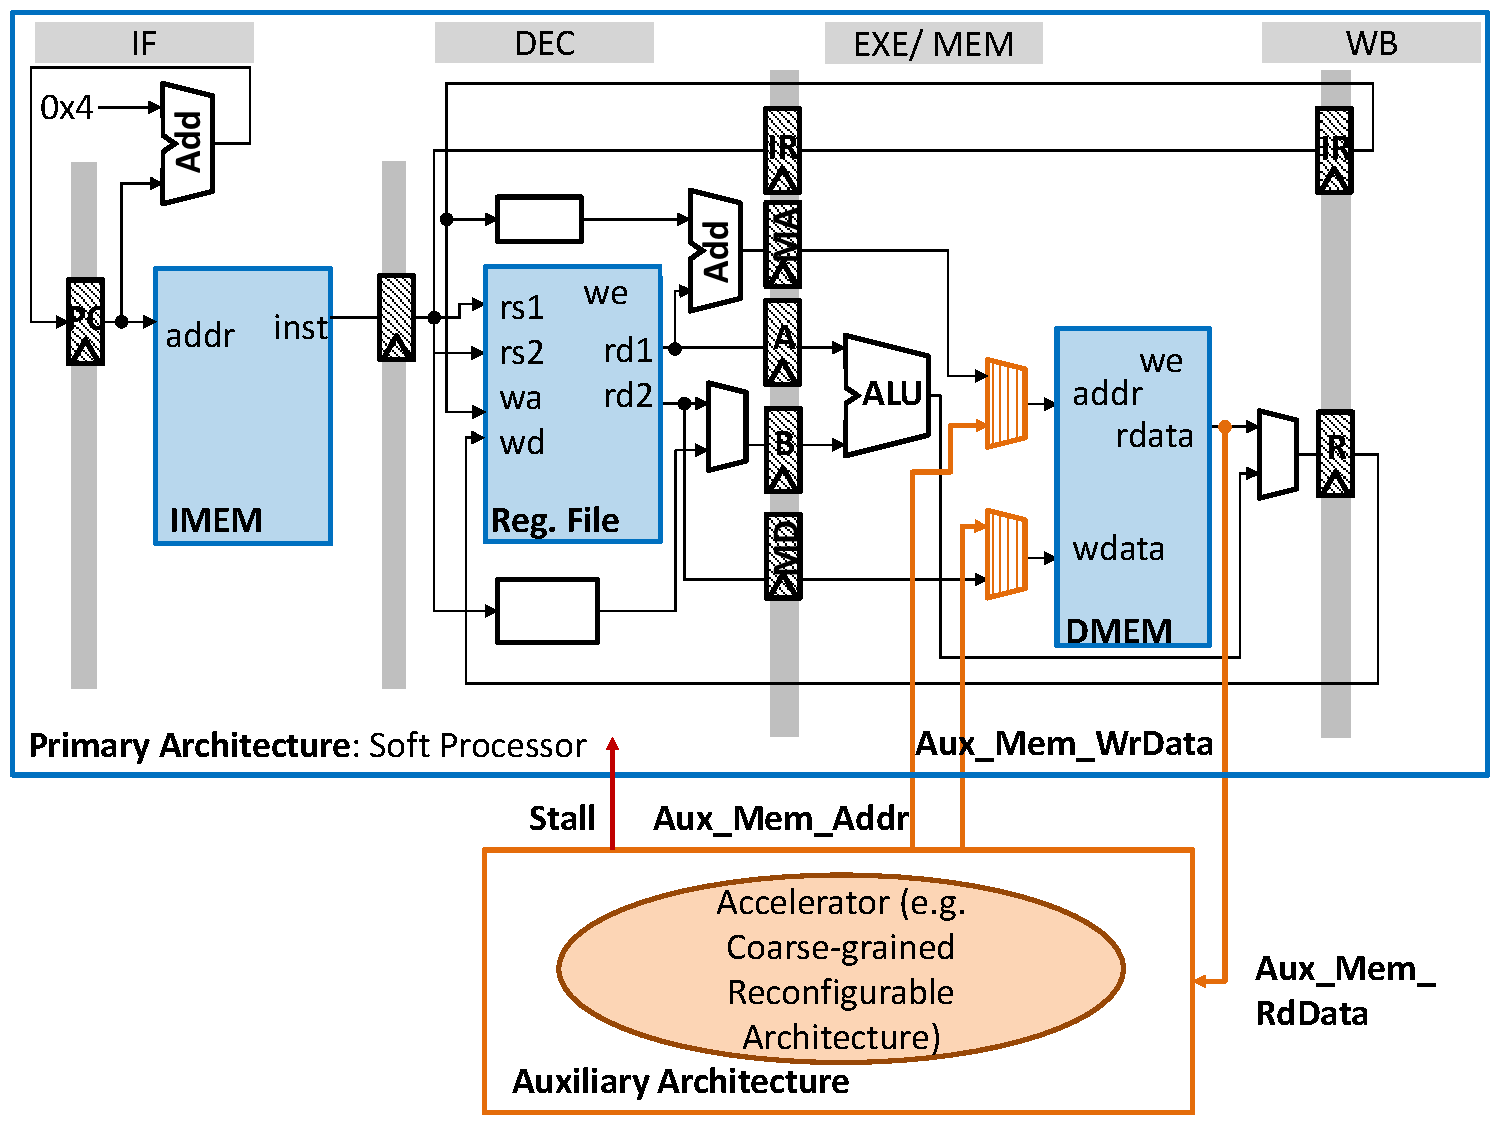
\includegraphics[width=3.3in]{tightly_coupled}
    \caption{High-level diagram of the proposed tightly-coupled architecture.}
    \label{fig:tightly}
\end{figure}

\figref{fig:tightly} displays a high-level diagram of the proposed tightly-coupled architecture. This design consists of two entities where an accelerator can be integrated with the single-issue, in-order processor pipeline by sharing the data memory (DMEM). To ensure correct execution flow, control signal is fed from the accelerator to the processor control path so that the pipeline is stalled correctly when the accelerator is carrying out execution.

\subsection{The Soft Processor}
%As the processor is usually responsible for 10\% time of the entire FPGA overlay execution, it is imperative to have the processor being relatively small in size. 
%As the processor is implemented as part of the FPGA overlay framework, it is imperative to have the processor being relatively small in size. 

In order to reduce substantial resource consumption while maintaining certain efficiency, the soft processor is designed as a 4-stage pipeline by integrating the execution-stage and memory-stage together. This eliminates the load-use hazard where a LOAD instruction is followed by an instruction that uses the value which is just transferred from DMEM to Register File.

In spite of the above advantage, since the memory-stage is now merged with the execution-stage and the memory address needs to be ready before the load/store instruction reaches DMEM, an extra 32-bit adder is placed at the end of the decode-stage. This could incur extra resource consumption and additional pipeline delay.

We found that, from the synthesis results, the proposed 4-stage processor consumes 18\% fewer amounts of FPGA registers and LUTs when compared with the traditional 5-stage pipeline. We believe that this reduction is important for portability and compatibility concerns, especially when the soft processor is ported onto the legacy FPGA devices which could be intrinsically small in size. Also, the additional delay incurred by the extra adder could be partly compensated  by the two additional multiplexers which are placed in front of DMEM.

Moreover, as the benefit of using a virtual layer of overlay architecture on FPGA rests on improving designer's productivity while providing certain customization capabilities, the proposed soft processor can also be customized in terms of the IMEM and DMEM size. Developers can change the memory sizes by modifying a few lines of macro or execute a program that comes along with the soft processor design package.

It is important to note that, in order to further minimize FPGA resource consumptions, components that are not strictly necessary for processor overlay execution are removed from the current implementation. These components include the Control Status Registers (CSR) and their corresponding logic. Future versions of the processor implementation will incorporate the CSR back and will provide tools to allow developers to remove them during the processor customization.

\begin{table}
\begin{center}
\caption{The format of \code{BAA} instruction.}
\label{tab:baa}
%\vspace{5pt}
\renewcommand{\arraystretch}{0.75}% Tighter
\begin{tabular}{|c|c|c|c|c|}
\multicolumn{1}{c}{\code{31\hspace{9mm}20}}%2.3mm as 1 space
 & \multicolumn{1}{c}{\code{19\hspace{4mm}15}}
 & \multicolumn{1}{c}{\code{14\hspace{2mm}12}}
 & \multicolumn{1}{c}{\code{11\hspace{4mm}7}}
 & \multicolumn{1}{c}{\code{6\hspace{7mm}0}}\\
\hline
\code{imm[11:0]}&\code{rs1}&\code{funct3}&\code{-}&\code{opcode}\\
\hline

\multicolumn{1}{c}{\code{12}}
 & \multicolumn{1}{c}{\code{5}}
 & \multicolumn{1}{c}{\code{3}}
 & \multicolumn{1}{c}{\code{5}}
 & \multicolumn{1}{c}{\code{7}}\\

\multicolumn{1}{c}{\code{offset[11:0]}}
 & \multicolumn{1}{c}{\code{base}}
 & \multicolumn{1}{c}{\code{width}}
 & \multicolumn{1}{c}{\code{-}}
 & \multicolumn{1}{c}{\code{BAA}}\\
\end{tabular}
\end{center}
\end{table}

\begin{table}
\begin{center}
\caption{The format of \code{RPA} instruction.}
\label{tab:rpa}
%\vspace{5pt}
\renewcommand{\arraystretch}{0.75}% Tighter
\begin{tabular}{|c|c|c|c|c|}
\multicolumn{1}{c}{\code{31\hspace{9mm}20}}%2.3mm as 1 space
 & \multicolumn{1}{c}{\code{19\hspace{4mm}15}}
 & \multicolumn{1}{c}{\code{14\hspace{2mm}12}}
 & \multicolumn{1}{c}{\code{11\hspace{4mm}7}}
 & \multicolumn{1}{c}{\code{6\hspace{7mm}0}}\\
\hline
\code{imm[11:0]}&\code{rs1}&\code{funct3}&\code{-}&\code{opcode}\\
\hline

\multicolumn{1}{c}{\code{12}}
 & \multicolumn{1}{c}{\code{5}}
 & \multicolumn{1}{c}{\code{3}}
 & \multicolumn{1}{c}{\code{5}}
 & \multicolumn{1}{c}{\code{7}}\\

\multicolumn{1}{c}{\code{offset[11:0]}}
 & \multicolumn{1}{c}{\code{base}}
 & \multicolumn{1}{c}{\code{width}}
 & \multicolumn{1}{c}{\code{-}}
 & \multicolumn{1}{c}{\code{RPA}}\\
\end{tabular}
\end{center}
\end{table}

\subsection{The Tightly-coupled Architecture}
In order to support direct memory access and allow zero-overhead transfers of control, the soft processor is tightly-coupled with the hardware accelerator as illustrated in \figref{fig:tightly}.
In the proposed framework, Multiple Runtime Architecture Computer(MURAC) model~\cite{murac} is adopted to handle the transfer of control when the execution is switched from one architecture to another.

%In order to have the soft-processor tightly-coupled with the CGRA, we need to investigate how the execution can be switched from one architecture to another. In other words, the mechanisms involved during the transfer of control in runtime execution must be well-defined. This is to provide a unified programming model for designers and facilitate compilation and execution on the mixed-architecture in FPGA overlay.

%\subsubsection{MURAC}
%In the proposed framework, Multiple Runtime Architecture Computer (MURAC)~\cite{murac} is employed to implement the above mechanism. MURAC is a unified machine model that considers heterogeneous computing architecture system as a single idealized processor with morphable instruction execution units. That is, the idealized processor can morph its architecture anytime during the runtime for the sake of the performance benefits. It provides an abstraction to programmers by utilizing different computational architectures during runtime to a level similar to the ISA for a specific processor, which abstracts away the low-level details of the hardware structures.


The execution model of the tightly-coupled architecture follows naturally from the MURAC model where the proposed 4-stage pipeline is defined as the \emph{primary architecture} while the hardware accelerator is defined as the \emph{auxiliary architectures}. Switching between these two architectures in runtime is achieved by the Branch-Auxiliary Architecture (\code{BAA}) and Return-To-Primary-Architecture (\code{RPA}) machine instructions. Logically, a MURAC machine contains only one address space that is shared between two architectures.



\subsubsection{Custom Instruction-set Extension}
To apply MURAC machine for the proposed tightly-coupled architecture, custom instruction-set is used to implement the \code{BAA} and \code{RPA} instructions.

Custom instruction-set extension~\cite{riscv_spec} is an important feature in RISC-V \code{RV32I} in the sense that it provides opportunity for designers to integrate other hardware modules such as accelerators onto a standard RISC-V processor. It also provides a unified programming model along various and future RISC-V processor designs, which makes it easier to leverage software development efforts for the ISA toolchain during the processor customization process.


\subsubsection{\code{BAA} and \code{PRA} Instructions Format}
In the proposed architecture, opcode space \emph{custom-0} is selected to implement the \code{BAA} and \code{RPA} instructions. The format of this opcode is defined to be \code{inst[6:0]==0001011}. For the benefits of regularity and simplicity of the decoding hardware, both instructions follow the format of I-type instruction.

\tabref{tab:baa} displays the the format of \code{BAA} instruction which resembles the format as in \code{LOAD} instruction. The fields \code{base} and \code{offset} are added together to form a memory address location. It represents an address location that points to an array of data. This address is passed to the auxiliary architecture, i.e. accelerator during the execution of the \code{BBA} instruction.

The array passed to the auxiliary architecture acts like the command line arguments in any \code{C/C++} program. It stores up the data that is needed by accelerator. The first data represents the number of elements inside the array.


The field \code{width}, on the other hand, is used to distinguish between the \code{BAA} and \code{RPA} instructions, as they share similar encoding. The format of the \code{RPA} instruction is shown in \tabref{tab:rpa}.

The fields \code{base} and \code{offset} in \code{RPA} instruction are added together to form a return memory address. This instruction acts like a return instruction where the program is unconditionally jumped to \code{\code{base+offset}}. Currently, the processor will branch to the address \code{(PC+4)} after the auxiliary architecture finishes its execution. %However, in some scenarios, the processor can adopt the broad definition of an instruction to represent any entity that configures  the machine so as to carry out proper computation. In this case, an FPGA configuration bitfile may be treated as an ultra-long instruction~\cite{quickdough, dehon}, which would make the return address to be \code{PC+length(bitfile)}. 





\subsubsection{Modifications of the Soft Processor}
In the control-path, extra control registers are defined to decode the \code{BAA} and \code{RPA} instructions. These registers are used to recognize the custom instruction with the help of comparators. In addition, stall signals are fed from the auxiliary architecture to the control-path so that the processor would not be executing once the control is passed to accelerator.

On the other hand, when the execution is branched to the auxiliary architecture, the processor pipeline is stalled and components on the data-path such as \code{DMEM} would not be accessed. This makes resource sharing between two architectures possible. In the proposed architecture, \code{DMEM} is designed to be shared with the accelerator. A number of multiplexers are added before the inputs of the \code{DMEM} and the output of \code{DMEM} is also fed to the auxiliary architecture. The control path would assert the correct \code{sel} signal for the multiplexers when the control is branched to auxiliary architecture.

\section{Experiments \& Measurements}
\label{sec:evaluation}

To study the design implications of the  proposed framework, a set of real-life applications was programmed and run on the tightly-coupled architecture. %Then the obtained performance of the benchmark was further compared with that achieved through pure hardware and pure software respectively. 
In addition, the soft processor was also benchmarked and compared with an existing similar RSIC-V design. Finally, resource consumption and design portability of the soft processor were evaluated to warrant the merit of the proposed framework as FPGA overlay.

\begin{table}
\begin{center}
  \caption{Parameters and configurations of the benchmarks.}
  \label{tab:tight_benchmark}

  \scriptsize
	\begin{tabular}{m{10mm}|m{16mm}|m{15mm}|m{27mm}}
    \toprule
	\bf MM  &  \bf FIR & \bf KM & \bf SE \\ 
	\hline	
	Matrix Size & \# of Input/ \# of Taps+1 & \# of Nodes/ Centroids/ Dimension & \# of Vertical Pixels/ \# of Horizontal Pixels\\
	\hline	
	100$\times$100 & 10000/50 & 5000/4/2 & (128+2)/(128+2)\\
    \bottomrule    
  \end{tabular}
\end{center}
\end{table} 

\begin{table}
\begin{center}
  \caption{The loop kernels were unrolled by the following factors before transferring to the auxiliary architecture for acceleration.}
  \label{tab:tight_unrolled}

  \scriptsize
	\begin{tabular}{m{12mm}|m{12mm}|m{11mm}|m{10mm}|m{16mm}}
    \toprule
	 & \bf MM  &  \bf FIR & \bf KM & \bf SE \\ 
	\hline	
	Full Loop & 100$\times$100$\times$ 100 & 10000$\times$ 50 & 5000$\times$ 4$\times$2 & (128+2)$\times$ (128+2)$\times$3$\times$3\\
	\hline	
	Unrolling & 1$\times$5$\times$100 & 50$\times$50 & 125$\times$4$\times$2 & 16$\times$16$\times$3$\times$3\\
    \bottomrule    
  \end{tabular}
\end{center}
\end{table} 



\subsection{Evaluation of the Tightly-coupled Architecture}
\subsubsection{Experimental Setup}
%In order to perform an accurate evaluation of the proposed architecture, the set of applications that are used to benchmark QuickDough~\cite{quickdough_fsp, quickdough} are used in this experiment. These benchmarks are essentially loop kernels which include 
Four real-life applications including matrix-matrix multiplication (MM), finite impulse response (FIR) filter, K-mean clustering algorithm (KM) and Sobel edge detector (SE) were taken as the benchmark to evaluate the tightly-coupled architecture. These applications are essentially loop kernels which are highly parallelizable and can be mapped to FPGA for performance acceleration. The parameters of the benchmark are listed in \tabref{tab:tight_benchmark}.

To understand the underlying influence of the tightly-coupled architecture (\textsc{Tightly-coupled}), the inner loop nest in each application was partially unrolled. Detailed loop unrolling configurations can be found in \tabref{tab:tight_unrolled}. The unrolled loop body was executed on a handcrafted hardware design (auxiliary architecture) for acceleration while miscellaneous loop controls and the boundary conditions that could not be covered by the accelerators were executed on the soft processor (primary architecture). The software was written in C and compiled with option \code{-O0}. 

Meanwhile, we also provided a pure hardware implementation (\textsc{HW}) and a pure software implementation (\textsc{SW}) for each of the applications for comparison. Basically, \textsc{HW} had the whole application implemented on FPGA with handcrafted hardware design. It can process not only the loop body but also the loop control as well as the boundary condition. Therefore, the execution can be done entirely on FPGA without the interventions from the soft processor. \textsc{SW} simply ignored the accelerator and had the whole application running on the proposed soft processor. The corresponding software was written in C and compiled with option \code{-O0}. 

Finally, we assumed that every piece of data was already cached in DMEM so as to eliminate the influence from the memory and maximize the impact of the soft processor architecture on the overall execution.
%in order to eliminate the influence from the memory hierarchy, we assumed that every piece of data was already cached in DMEM, which also maximizes the impact of the soft processor architecture on the overall execution.


%As mentioned in \secref{sec:implementation}, computational intensive kernels are mapped to the CGRA while the rest of the execution is handled by the soft processor according to the 90/ 10 locality rule. Therefore, in this experiments, the unrolled loop body is directed to the auxiliary architecture for acceleration while the miscellaneous loop controls and the boundary conditions are directed to the primary architecture, i.e. the soft processor to perform execution.

%However, in order to understand the underlying influence of the tightly-coupled architecture (\code{Tightly-coupled}), instead of using CGRA as the auxiliary architecture, handcrafted hardware design are used to accelerate the unrolled loop kernels. 


%In addition, in order to study the performance gain when compared with traditional software execution, C  programs for the above benchmarks are also written and they are executed on the official RISC-V Zscale core distributed by UC Berkeley~\cite{zscale}.

%Note that both \code{Tightly-coupled} and \code{HW} are running at \SI{50}{\mega\hertz} while the Zscale core is simulated at its maximum frequency \SI{500}{\mega\hertz}. The C program for the soft processor and the Zscale core is compiled with the option \code{-O0}.

\begin{figure}
    \centering
    \begin{subfigure}{0.23\textwidth}
        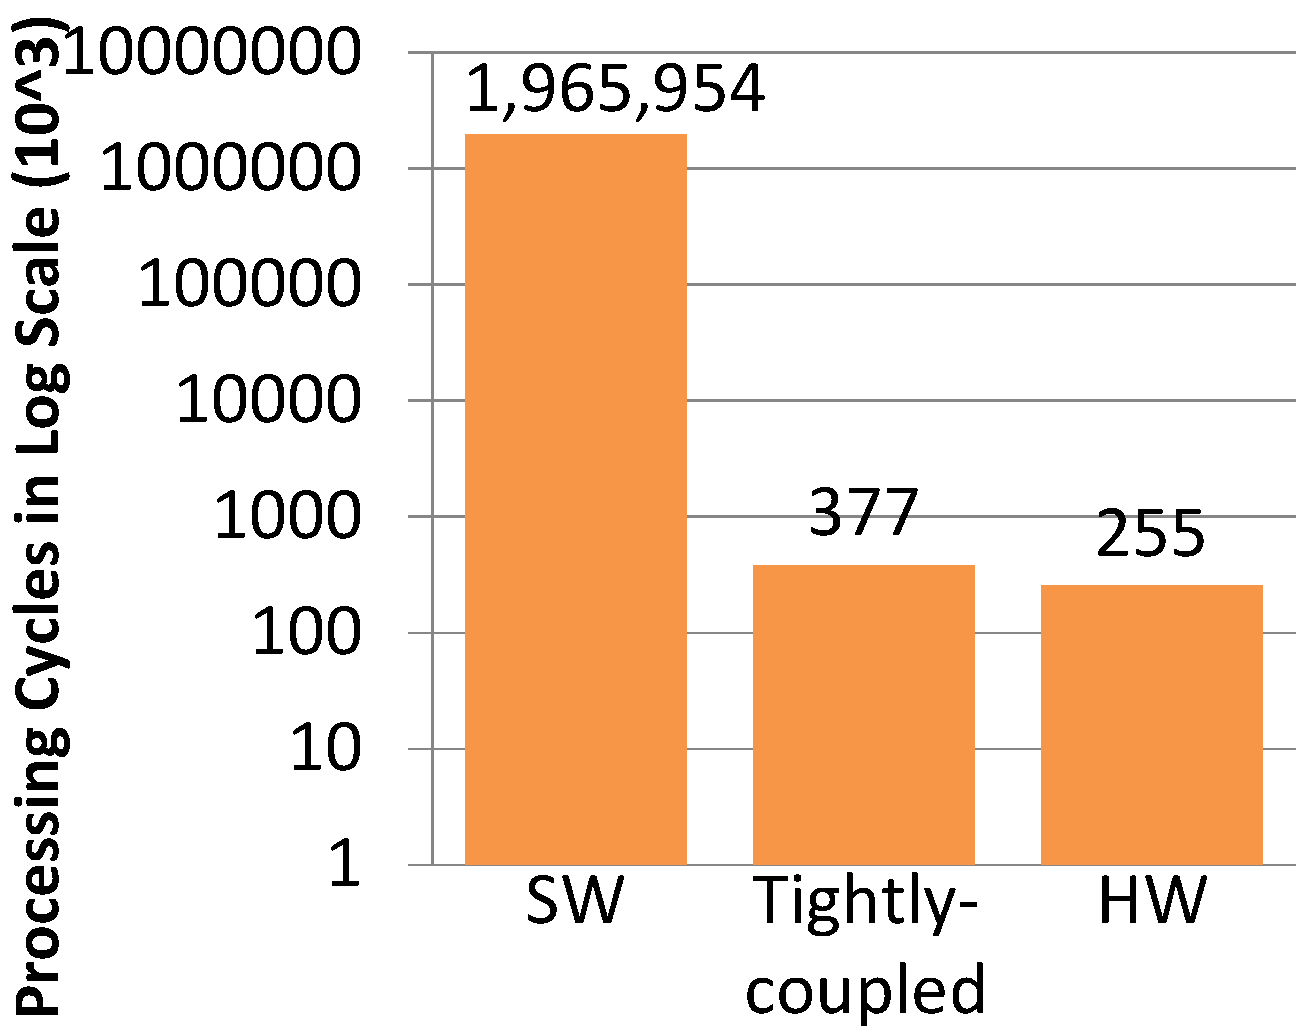
\includegraphics[width=\textwidth]{MM}
        \caption{MM}
        \label{fig:MM}
    \end{subfigure}
    ~ %add desired spacing between images, e. g. ~, \quad, \qquad, \hfill etc. 
      %(or a blank line to force the subfigure onto a new line)
    \begin{subfigure}{0.23\textwidth}
        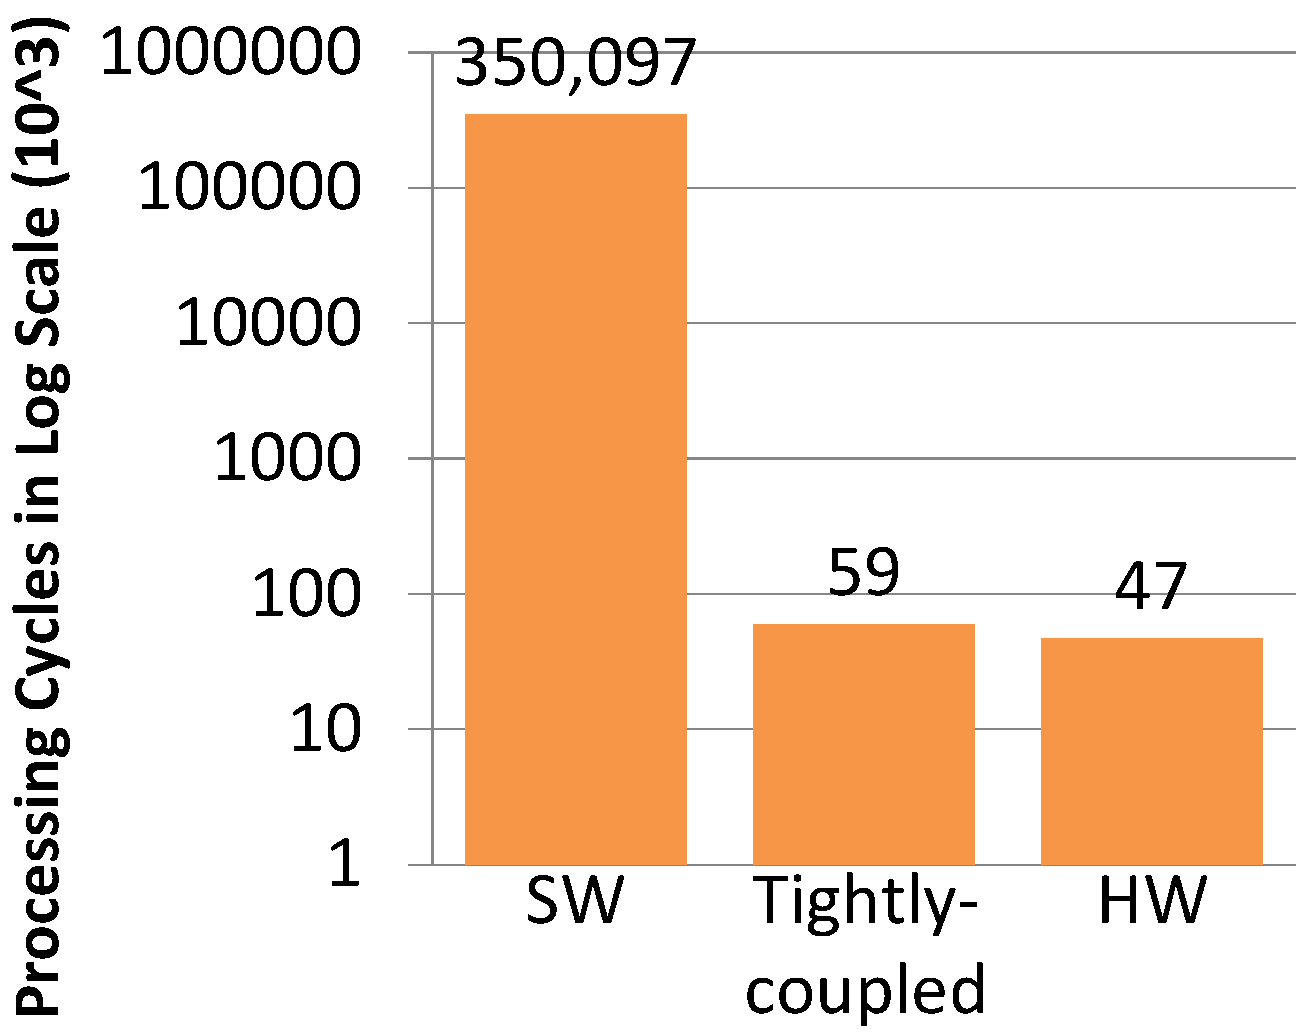
\includegraphics[width=\textwidth]{Fir}
        \caption{FIR}
        \label{fig:FIR}
    \end{subfigure}
    %\hfill
    
    ~ %add desired spacing between images, e. g. ~, \quad, \qquad, \hfill etc. 
    %(or a blank line to force the subfigure onto a new line)
    \begin{subfigure}{0.23\textwidth}
        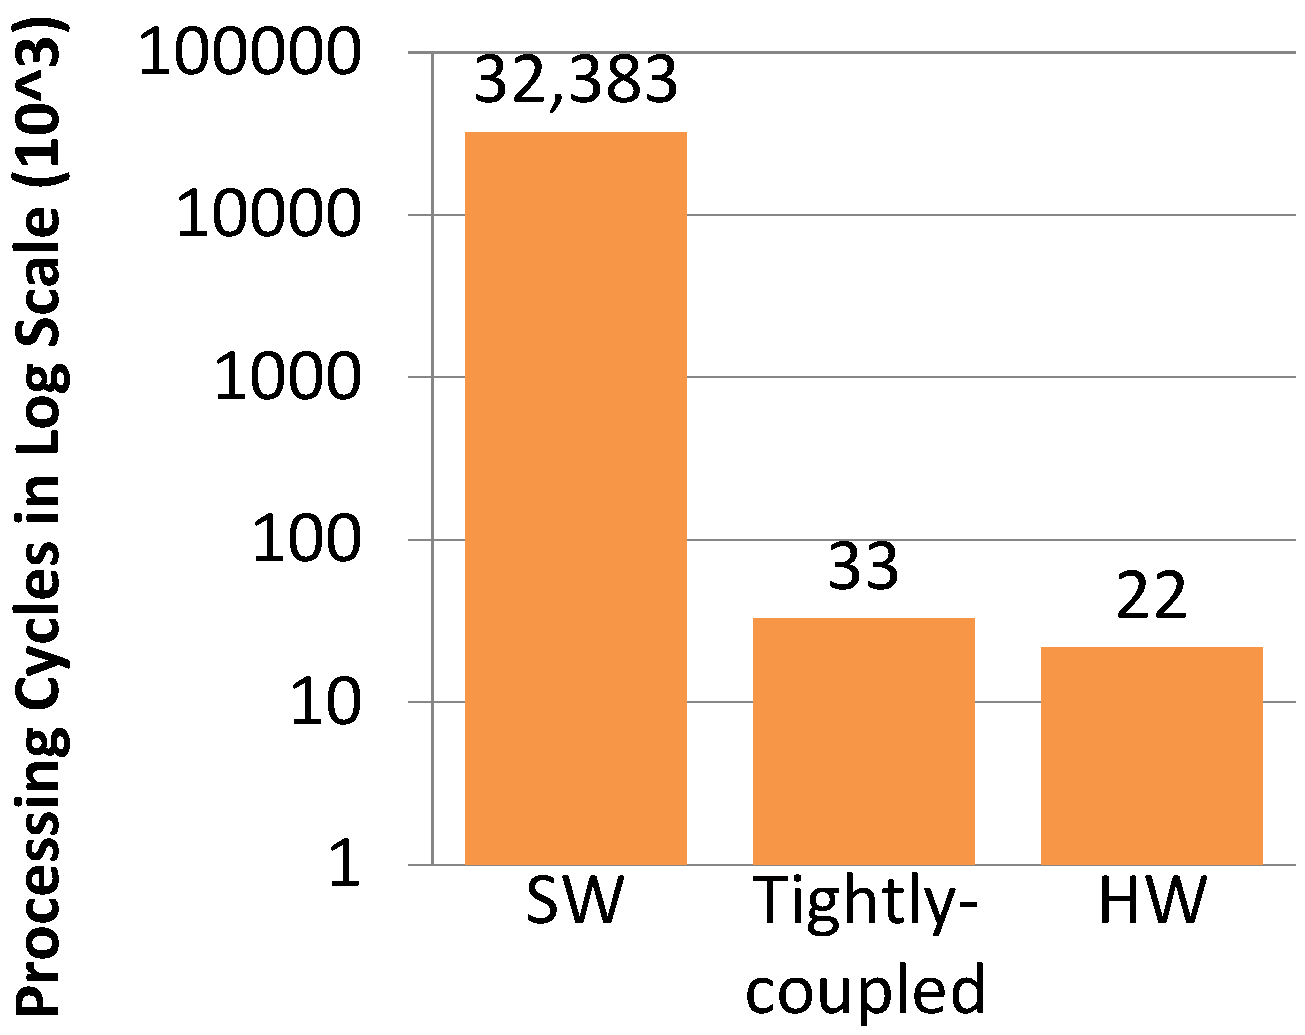
\includegraphics[width=\textwidth]{Kmean}
        \caption{KM}
        \label{fig:KM}
    \end{subfigure}
    \begin{subfigure}{0.23\textwidth}
        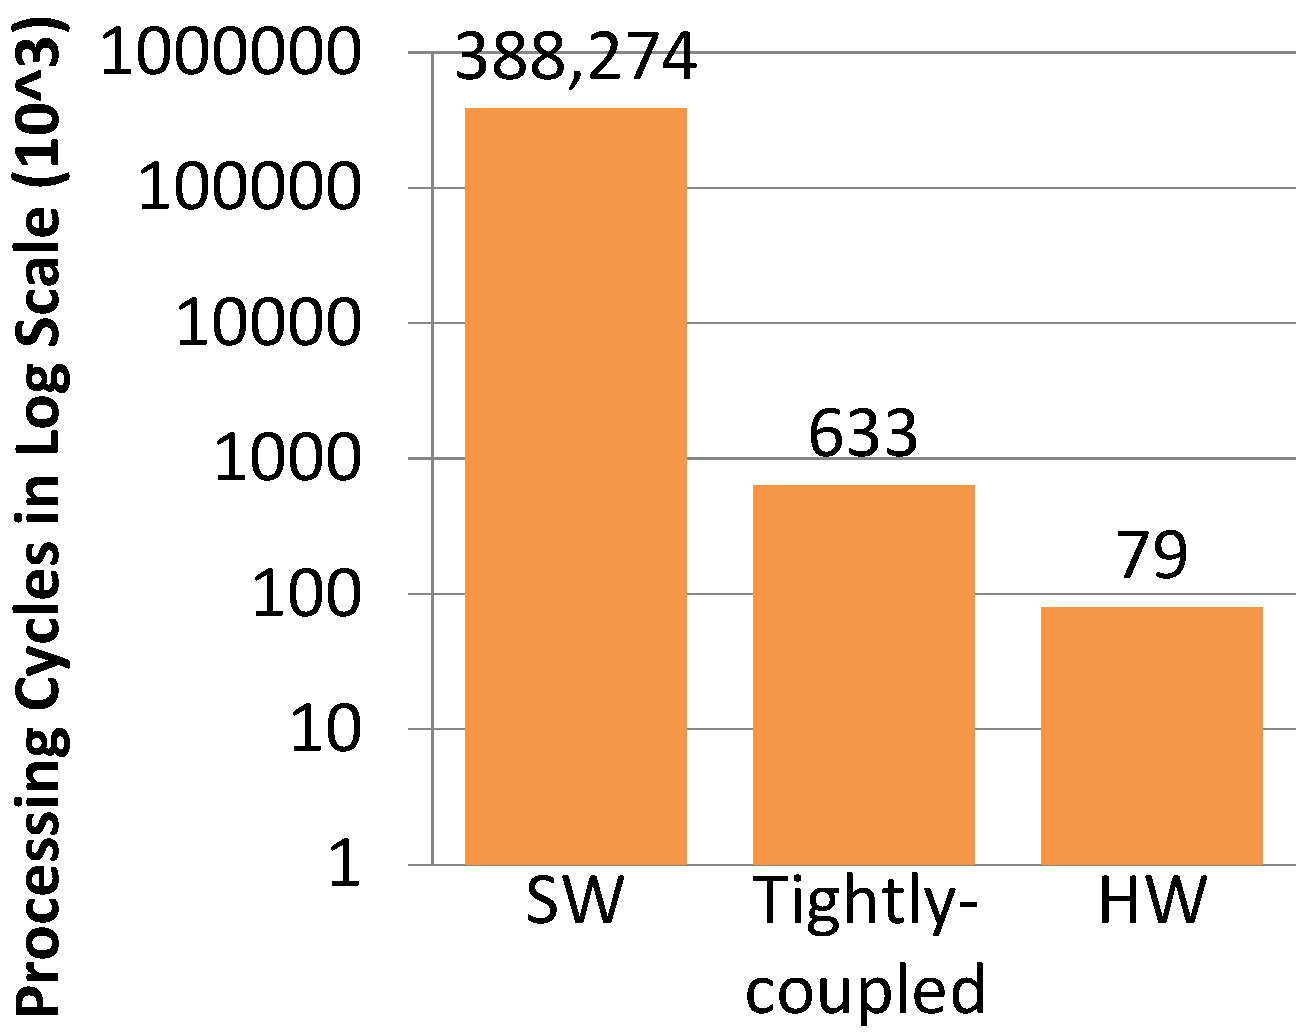
\includegraphics[width=\textwidth]{Sobel}
        \caption{SE}
        \label{fig:SE}
    \end{subfigure}
    \caption{The performance of \textsc{SW} versus \textsc{Tightly-coupled} versus \textsc{HW}. }\label{fig:tight_bench}
\end{figure}

\subsubsection{Results \& Analysis}
%Performance results of \textsc{SW} versus \textsc{Tightly-coupled} versus \textsc{HW} are displayed in \figref{fig:tight_bench} in terms of processing cycles.

As shown in \figref{fig:tight_bench}, the tightly-coupled architecture achieves similar performance when compared with \textsc{HW} in most of the benchmarks. In particular, it is found that the execution of MM, FIR and KM on \textsc{Tightly-coupled} exhibits comparable performance to that on \textsc{HW}. The main reason is that these applications only need the soft processor to handle the loop control which takes a small amount of time while they rely on the FPGA accelerators to handle the most time-consuming computing.
 
%achieve a speedup more than 60$\times$ since the soft processor is only required to handle the loop control. In addition, the handcrafted hardware designs for the unrolled loop kernels are fully-pipeline implementations that take inputs every clock cycle, therefore the overall execution latency can be extensively shortened.

In the case of SE, however, the number of processing cycles needed in \textsc{Tightly-coupled} is significantly more than that in \textsc{HW}. Such performance discrepancy is mainly caused by the following two factors. First, the boundary conditions in SE, i.e. the edge pixels, could not be covered by the auxiliary architecture for acceleration. Therefore a relatively large amount of elements (516 in this case) had to be handled by the soft processor. This would undoubtedly increase the overall execution latency. Second, SE needed the soft processor to perform a large amount of multiplication to calculate the correct memory location for a particular pixel and the entire execution latency will be lengthened consequently, especially when \code{RV32I} does not include a multiply instruction. This problem can be alleviated by extending the ISA to \code{RV32IM} and incorporating a multiplier in the soft processor design, which will be supported in the future as one of the customization parameters in the proposed framework.

%However, in the case of SE, the speedup is relatively limited and the performance gain is only about 4$\times$. The reason for such insignificant speedup is mainly because of the following two reasons. 


%\Hsection{Matrix-matrix Multiplication} The input is two $100 \times 100$ matrix (\code{M1}), (\code{M2}) and output is a $100 \times 100$ matrix (\code{M3}). 


\subsection{Evaluation of the Soft Processor}
As mentioned in \secref{sec:introduction}, though the soft processor is mostly responsible for irregular data processing and controlling over the accelerator, it is still important to have the processor to maintain sufficient efficiency while keeping the area consumption minimal. 

\subsubsection{Experimental Setup}

\begin{table}
\begin{center}
  \caption{Resource consumption and maximum frequency of the proposed soft processor versus ORCA RISC-V core.}
  \label{tab:guy_resource}
  \small
%  \begin{tabular}{p{0.8in}p{0.4in}p{0.4in}p{0.4in}p{0.4in}p{0.4in}p{0.4in}}
  \begin{tabular}{m{12mm}m{3mm}m{3mm}m{3mm}m{3mm}m{3mm}m{3mm}m{14mm}}%{lSSSSSSS}
    \toprule
%    \multirow{2}{*}{\textbf{Modules}} & \multicolumn{3}{c}{\textbf{Logic}}  &  \multicolumn{3}{c}{\textbf{Utilization}}  & FF & (\%) & BRAM &FF & LUT & BRAM\\\midrule
    \textbf{Designs} & 
    \multicolumn{2}{c}{ \begin{minipage}{0.55in}\textbf{Slice Registers}\end{minipage}}& 
    \multicolumn{2}{c}{\begin{minipage}{0.45in}\textbf{Slice LUTs}\end{minipage}}& 
    \multicolumn{2}{c}{\begin{minipage}{0.45in}\textbf{Block RAM}\end{minipage}} & 
    \begin{minipage}{0.9in}\textbf{Max. Freq.}\end{minipage}\\\midrule
      \begin{minipage}{0.5in}Proposed Soft Processor\end{minipage} & \num{334} & \SI{\sim0}{\percent} &  \num{1279} & \SI{2}{\percent} &  \num{6} & \SI{4}{\percent} & \SI{147.929}{\mega\hertz}\\\midrule
            
      \begin{minipage}{0.5in}ORCA RISC-V core\end{minipage} & \num{615} & \SI{\sim0}{\percent} &  \num{1438} & \SI{2}{\percent} &  \num{1} & \SI{\sim0}{\percent} & \SI{199.322}{\mega\hertz}\\\bottomrule
   
  \end{tabular}
  \end{center}
\end{table}


\begin{table}
\begin{center}
  \caption{Processing cycles and the execution latency of the four benchmarks on the proposed soft processor and ORCA RISC-V core.}
  \label{tab:guy_benchmark}
\renewcommand{\arraystretch}{1.5}
  \small
	\begin{tabular}{lcll}
    \toprule
	 \bf Designs & \bf Benchmarks  &  \bf \# of Cycles & \bf Latency\\ 
	 \hline	
	\multirow{4}{*}{\begin{minipage}{0.5in}Proposed Soft Processor\end{minipage}}
	 & MM & 1965954155 & \SI{13.29}{\second} \\
	 & FIR & 350096784 & \SI{2.37}{\second} \\
	 & KM & 32382531 & \SI{0.22}{\second} \\
	 & SE & 388273610 & \SI{2.62}{\second} \\
	\hline	
	\multirow{4}{*}{\begin{minipage}{0.5in}ORCA RISC-V core\end{minipage}}
	 & MM & 2868605367 & \SI{14.39}{\second} \\
	 & FIR & 503309228 & \SI{2.53}{\second} \\
	 & KM & 46286121 & \SI{0.23}{\second} \\
	 & SE & 566543126 & \SI{2.84}{\second} \\

    \bottomrule    
  \end{tabular}
\end{center}
\vspace{-2em}
\end{table} 

In order to study the efficiency of the proposed soft processor, we compared the proposed 4-stage pipeline processor with ORCA RISC-V core from VectorBlox Computing Inc.~\cite{vectorblox}. ORCA core is known as an optimized RISC-V design on FPGA that implements a 4-stage pipeline, which is most close to the proposed soft processor. Both design were implemented on Artix 7 xc7a100t-1csg324 using Xilinx ISE 14.3. Then $f_{MAX}$ as well as the resource consumption of the implementations are obtained. Meanwhile, the number of cycles that are needed to compute the benchmark are obtained from the RTL simulation.   

\subsubsection{Results \& Analysis}
\tabref{tab:guy_resource} and \tabref{tab:guy_benchmark} display the resource consumption and the performance of the proposed soft processor versus ORCA core. The percentage in \tabref{tab:guy_resource} are relative to all the available resources of the targeted FPGA device.

From these tables, we can see that the proposed soft processor typically occupies less area while at the same time providing slightly higher processing speed. The only resource that the proposed soft processor consumes more than that of ORCA core is the on-chip block RAM. This is mainly due to the existence of the IMEM and DMEM which are inferred as block RAM in the proposed processor. Such memory modules do not exist in ORCA core and hence that explains the discrepancy in block RAM consumption.


\subsection{Portability and Compatibility Considerations}
One of the major advantages of FPGA overlay is to raise the device abstraction by providing a virtual layer that is conceptually located between the user applications and the physical FPGA. Therefore, to add the soft processor to the same overlay framework with that of the accelerator, the processor must be able to support cross-vendors and cross-platforms FPGAs to ensure the device portability and compatibility.

In view of this, we have designed the processor in a generic manner such that the 4-stage pipeline design can be synthesized across various platforms ranging from Spartan-3 to Virtex-7 and Cyclone IV to V. \tabref{tab:big_resource} displays the resource consumption and the $f_{MAX}$ of the soft processor implementations on both the high-end and low-end FPGA devices. Again, the percentage in the table is relative to all the available resources on the target FPGA device.


\begin{table*}
\begin{center}
  \caption{Resource consumption and maximum frequency of the proposed soft processor on high-end and low-end FPGA devices across various generations.}
  \label{tab:big_resource}
  \renewcommand{\arraystretch}{1.3}
  \small
%  \begin{tabular}{p{0.8in}p{0.4in}p{0.4in}p{0.4in}p{0.4in}p{0.4in}p{0.4in}}
  \begin{tabular}{lSSSSSSS}
    \toprule
%    \multirow{2}{*}{\textbf{Modules}} & \multicolumn{3}{c}{\textbf{Logic}}  &  \multicolumn{3}{c}{\textbf{Utilization}}  & FF & (\%) & BRAM &FF & LUT & BRAM\\\midrule
    \textbf{Devices} & \multicolumn{2}{c}{\textbf{Slice Flip Flops}}& \multicolumn{2}{c}{\textbf{4 Input LUTs}}& \multicolumn{2}{c}{\textbf{RAMB16s}} & \textbf{Max. Freq.}\\\midrule
      Spartan3 xc3s50-5vq100 & \num{304} & \SI{19}{\percent} &  \num{1461} & \SI{95}{\percent} &  \num{2} & \SI{50}{\percent} & \SI{76.127}{\mega\hertz}\\
      
      Virtex4 xc4vfx140-11ff1517 & \num{248} & \SI{\sim0}{\percent} &  \num{1344} & \SI{1}{\percent} &  \num{4} & \SI{\sim0}{\percent} & \SI{157.351}{\mega\hertz}\\\midrule
      
      \textbf{Devices} & \multicolumn{2}{c}{\textbf{Slice Registers}}& \multicolumn{2}{c}{\textbf{Slice LUTs}}& \multicolumn{2}{c}{\textbf{Block RAM }} & \textbf{Max. Freq.}\\\midrule
      Virtex5 xc5vlx30-1ff324 & \num{280} & \SI{1}{\percent} &  \num{1081} & \SI{5}{\percent} &  \num{2} & \SI{6}{\percent} & \SI{184.735}{\mega\hertz}\\
      
      Virtex5 xc5vlx155t-3ff1738 & \num{266} & \SI{\sim0}{\percent} &  \num{1070} & \SI{1}{\percent} &  \num{2} & \SI{\sim0}{\percent} & \SI{231.913}{\mega\hertz}\\\midrule      
      

      Spartan6 xc6slx4-2tqg144 & \num{369} & \SI{7}{\percent} &  \num{1296} & \SI{61}{\percent} &  \num{10} & \SI{83}{\percent} & \SI{88.355}{\mega\hertz}\\
      
      Virtex6 xc6vhx380t-3ff1923 & \num{321} & \SI{\sim0}{\percent} &  \num{1263} & \SI{\sim0}{\percent} &  \num{6} & \SI{\sim0}{\percent} & \SI{203.198}{\mega\hertz}\\\midrule   
      
      Artix7 xc7a100t-1csg324 & \num{334} & \SI{\sim0}{\percent} &  \num{1279} & \SI{2}{\percent} &  \num{6} & \SI{4}{\percent} & \SI{147.929}{\mega\hertz}\\
      
      Virtex7 xc7vx690t-3ffg1927 & \num{318} & \SI{\sim0}{\percent} &  \num{1280} & \SI{\sim0}{\percent} &  \num{6} & \SI{\sim0}{\percent} & \SI{268.666}{\mega\hertz}\\\midrule 
  
  
    \textbf{Devices} & \multicolumn{2}{c}{\textbf{Logic Registers}}& \multicolumn{2}{c}{\textbf{Logic Elements}}& \multicolumn{2}{c}{\textbf{Memory Bits}} & \textbf{Max. Freq.}\\\midrule
      Cyclone IV EP4CE6F17C8 & \num{284} & \SI{4}{\percent} &  \num{1890} & \SI{30}{\percent} &  \SI{165888}{\kilo\bit} & \SI{60}{\percent} & \SI{68.43}{\mega\hertz}\\
      
      Cyclone IV EP4CGX75DF27C6 & \num{284} & \SI{3}{\percent} &  \num{1890} & \SI{3}{\percent} &   \SI{165888}{\kilo\bit} & \SI{4}{\percent}  & \SI{93.07}{\mega\hertz}\\\midrule    
  
  
  
      
    \textbf{Devices} & \multicolumn{2}{c}{\textbf{Logic Registers}}& \multicolumn{2}{c}{\textbf{ALM}}& \multicolumn{2}{c}{\textbf{Memory Bits}} & \textbf{Max. Freq.}\\\midrule
      Cyclone V 5CEBA2F17C8 & \num{284} & \SI{2}{\percent} &  \num{784} & \SI{8}{\percent} &  \SI{165888}{\kilo\bit} & \SI{9}{\percent} & \SI{73.5}{\mega\hertz}\\
      
      Cyclone V 5CGXFC7D6F31C6 & \num{284} & \SI{1}{\percent} &  \num{791} & \SI{1}{\percent} &   \SI{165888}{\kilo\bit} & \SI{2}{\percent}  & \SI{102.76}{\mega\hertz}\\\midrule  
   
  \end{tabular}
  \end{center}
\end{table*}

\section{Related Work}
To improve the productivity of FPGA designers, researchers have approached the problem both by increasing the abstraction level and by reducing the compilation time.

In the first case, decades of research in FPGA high-level synthesis have already demonstrated their indispensible role in promoting FPGA design productivity \cite{cong2011high}. Numerous design languages and environments \cite{cardoso2010compiling} have been developed to allow designers to focus on high-level functionality instead of low-level implementation details. 

While high-level abstraction may help a designers express the desired functionality, the low-level compilation time spent on synthesis, map, and place-and-route for FPGAs remains a major hindrances to designs' productivity. Researchers have approached the problem from many angles, such as through the use of pre-compiled hard macros \cite{lavin2011} in the tool flow, the use of a partial reconfiguration, modular design flow \cite{Frangieh2010}, and the use of coarse-grained reconfigurable fabrics upgrading the configurability from bit-level to word-level \cite{coole2010intermediate} \cite{ferreira2011fpga}. 

%Particularly, the authors in \cite{coole2010intermediate} proposed to implement an intermedia fabrics (IF) as an virtual device on top of commerical-off-the-shelf (COTS) FPGA devices. The IF has computational units connected through the connection boxes and switch boxes and it is more like a traditional FPGA with word-level configurability. It hides much of the complexity of fine-grained COTS FPGA device and enables great speedup of the placement and routing as well as portability over different FPGA devices. This method follows traditional FPGA design flow, but the idea building an intermedia virtual fabrics over COTS device to reduce the complexity of FPGA synthesis and mapping is meanlingful. The authors in \cite{ferreira2011fpga} developed a heterogeneous CGRA as IF to further reduce the compilation time and improve the performance at the same time. 

Finally, the use of parameterizable VLIW processor array \cite{kissler2006dynamically} and even the many-core processors \cite{Lebedev2010} as a template to FPGA design has also been proposed demonstrating improve productivity with moderate performance degradation.

Building on top of many of the above ideas, we have opted to utilize a fully synchronous soft coarse-grained reconfigurable array as an intermediate step to compiling high-level compute intensive application. Productivity is improved both from the vastly reduced compilation time, as well as from the high-level abstraction provided by the generic LLVM compiler framework we utilized as front-end.

\section{Conclusion} \label{sec:Conclusion}
In this work, we propose to replace the forward computing on GPPs with accelerator 
computing during training and have both the computing 
errors and the application data learned in the neural network models. 
In addition, we opt to protect critical neural layers to reduce the negative 
influence of computing errors.  
With the proposed resilient neural network training, 
the prediction accuracy of the retrained neural network models improves significantly 
when computing errors appear. 


%\appendix
%\section{Acknowledgement}

%\begin{acks}
%  The authors would like to thank Sam Ho for providing the suggestions on
%  HLS design debugging and optimization as well as the SDAccel usage. 

%\end{acks}


\section*{Acknowledgment}
This work was supported in part by the Research Grants Council of Hong
Kong project ECS 720012E and the Croucher Innovation Award 2013. 

% For peer review papers, you can put extra information on the cover
% page as needed:
% \ifCLASSOPTIONpeerreview
% \begin{center} \bfseries EDICS Category: 3-BBND \end{center}
% \fi
%
% For peerreview papers, this IEEEtran command inserts a page break and
% creates the second title. It will be ignored for other modes.
\IEEEpeerreviewmaketitle






% An example of a floating figure using the graphicx package.
% Note that \label must occur AFTER (or within) \caption.
% For figures, \caption should occur after the \includegraphics.
% Note that IEEEtran v1.7 and later has special internal code that
% is designed to preserve the operation of \label within \caption
% even when the captionsoff option is in effect. However, because
% of issues like this, it may be the safest practice to put all your
% \label just after \caption rather than within \caption{}.
%
% Reminder: the "draftcls" or "draftclsnofoot", not "draft", class
% option should be used if it is desired that the figures are to be
% displayed while in draft mode.
%
%\begin{figure}[!t]
%\centering
%\includegraphics[width=2.5in]{myfigure}
% where an .eps filename suffix will be assumed under latex, 
% and a .pdf suffix will be assumed for pdflatex; or what has been declared
% via \DeclareGraphicsExtensions.
%\caption{Simulation results for the network.}
%\label{fig_sim}
%\end{figure}

% Note that the IEEE typically puts floats only at the top, even when this
% results in a large percentage of a column being occupied by floats.


% An example of a double column floating figure using two subfigures.
% (The subfig.sty package must be loaded for this to work.)
% The subfigure \label commands are set within each subfloat command,
% and the \label for the overall figure must come after \caption.
% \hfil is used as a separator to get equal spacing.
% Watch out that the combined width of all the subfigures on a 
% line do not exceed the text width or a line break will occur.
%
%\begin{figure*}[!t]
%\centering
%\subfloat[Case I]{\includegraphics[width=2.5in]{box}%
%\label{fig_first_case}}
%\hfil
%\subfloat[Case II]{\includegraphics[width=2.5in]{box}%
%\label{fig_second_case}}
%\caption{Simulation results for the network.}
%\label{fig_sim}
%\end{figure*}
%
% Note that often IEEE papers with subfigures do not employ subfigure
% captions (using the optional argument to \subfloat[]), but instead will
% reference/describe all of them (a), (b), etc., within the main caption.
% Be aware that for subfig.sty to generate the (a), (b), etc., subfigure
% labels, the optional argument to \subfloat must be present. If a
% subcaption is not desired, just leave its contents blank,
% e.g., \subfloat[].


% An example of a floating table. Note that, for IEEE style tables, the
% \caption command should come BEFORE the table and, given that table
% captions serve much like titles, are usually capitalized except for words
% such as a, an, and, as, at, but, by, for, in, nor, of, on, or, the, to
% and up, which are usually not capitalized unless they are the first or
% last word of the caption. Table text will default to \footnotesize as
% the IEEE normally uses this smaller font for tables.
% The \label must come after \caption as always.
%
%\begin{table}[!t]
%% increase table row spacing, adjust to taste
%\renewcommand{\arraystretch}{1.3}
% if using array.sty, it might be a good idea to tweak the value of
% \extrarowheight as needed to properly center the text within the cells
%\caption{An Example of a Table}
%\label{table_example}
%\centering
%% Some packages, such as MDW tools, offer better commands for making tables
%% than the plain LaTeX2e tabular which is used here.
%\begin{tabular}{|c||c|}
%\hline
%One & Two\\
%\hline
%Three & Four\\
%\hline
%\end{tabular}
%\end{table}


% Note that the IEEE does not put floats in the very first column
% - or typically anywhere on the first page for that matter. Also,
% in-text middle ("here") positioning is typically not used, but it
% is allowed and encouraged for Computer Society conferences (but
% not Computer Society journals). Most IEEE journals/conferences use
% top floats exclusively. 
% Note that, LaTeX2e, unlike IEEE journals/conferences, places
% footnotes above bottom floats. This can be corrected via the
% \fnbelowfloat command of the stfloats package.









% trigger a \newpage just before the given reference
% number - used to balance the columns on the last page
% adjust value as needed - may need to be readjusted if
% the document is modified later
%\IEEEtriggeratref{8}
% The "triggered" command can be changed if desired:
%\IEEEtriggercmd{\enlargethispage{-5in}}

% references section

% can use a bibliography generated by BibTeX as a .bbl file
% BibTeX documentation can be easily obtained at:
% http://mirror.ctan.org/biblio/bibtex/contrib/doc/
% The IEEEtran BibTeX style support page is at:
% http://www.michaelshell.org/tex/ieeetran/bibtex/
%\bibliographystyle{IEEEtran}
% argument is your BibTeX string definitions and bibliography database(s)
%\bibliography{IEEEabrv,../bib/paper}
%
% <OR> manually copy in the resultant .bbl file
% set second argument of \begin to the number of references
% (used to reserve space for the reference number labels box)

\bibliographystyle{IEEEtran}

\bibliography{IEEEabrv,olaf}




% that's all folks
\end{document}


